\documentclass[conference]{IEEEtran}
\usepackage{graphicx}
\usepackage{booktabs}
\usepackage{amsmath}
\usepackage{cite}
\usepackage{url}
\usepackage[hidelinks]{hyperref}
\graphicspath{{figs/}{../results/}}

% ---------------------------------------------------------------------------
% Milestone 2 (reproduction) numbers: fixed, from results/baseline_metrics.json
\newcommand{\RepAcc}{80.13$\pm$0.74}
\newcommand{\RepSens}{98.41$\pm$0.30}
\newcommand{\RepSpec}{49.66$\pm$1.94}
\newcommand{\RepPrec}{76.52$\pm$0.69}
\newcommand{\RepAUC}{92.89$\pm$0.24}
% Milestone 4 (ablation) numbers: run  python fill_macros.py  to refresh this block
%% BEGIN M4 MACROS (generated by fill_macros.py)
\newcommand{\AblZeroAcc}{TBD}
\newcommand{\AblZeroSens}{TBD}
\newcommand{\AblZeroSpec}{TBD}
\newcommand{\AblZeroPrec}{TBD}
\newcommand{\AblZeroAUC}{TBD}
\newcommand{\AblZeroTrain}{TBD}
\newcommand{\AblZeroVal}{TBD}
\newcommand{\AblZeroSeeds}{TBD}
\newcommand{\AblOneAcc}{TBD}
\newcommand{\AblOneSens}{TBD}
\newcommand{\AblOneSpec}{TBD}
\newcommand{\AblOnePrec}{TBD}
\newcommand{\AblOneAUC}{TBD}
\newcommand{\AblOneTrain}{TBD}
\newcommand{\AblOneVal}{TBD}
\newcommand{\AblOneSeeds}{TBD}
\newcommand{\AblTwoAcc}{TBD}
\newcommand{\AblTwoSens}{TBD}
\newcommand{\AblTwoSpec}{TBD}
\newcommand{\AblTwoPrec}{TBD}
\newcommand{\AblTwoAUC}{TBD}
\newcommand{\AblTwoTrain}{TBD}
\newcommand{\AblTwoVal}{TBD}
\newcommand{\AblTwoSeeds}{TBD}
\newcommand{\AblAllAcc}{TBD}
\newcommand{\AblAllSens}{TBD}
\newcommand{\AblAllSpec}{TBD}
\newcommand{\AblAllPrec}{TBD}
\newcommand{\AblAllAUC}{TBD}
\newcommand{\AblAllTrain}{TBD}
\newcommand{\AblAllVal}{TBD}
\newcommand{\AblAllSeeds}{TBD}
\newcommand{\DAUC}{TBD}
\newcommand{\DSpec}{TBD}
\newcommand{\DSens}{TBD}
\newcommand{\DAcc}{TBD}
\newcommand{\FPZero}{TBD}
\newcommand{\FPTwo}{TBD}
\newcommand{\FNZero}{TBD}
\newcommand{\FNTwo}{TBD}
\newcommand{\VerdictAUC}{TBD}
\newcommand{\VerdictSpec}{TBD}
\newcommand{\VerdictSens}{TBD}
\newcommand{\VerdictOverall}{TBD}
\newcommand{\OutcomeSummary}{TBD}
\newcommand{\MFilled}{no}
%% END M4 MACROS
% ---------------------------------------------------------------------------

\begin{document}

\title{Reproducing Frozen-InceptionV3 Pneumonia Detection on Pediatric Chest X-Rays, and Fine-Tuning Its Top Blocks}

\author{\IEEEauthorblockN{Vaiditya Tanwar}
\IEEEauthorblockA{Computer Vision Course Project (Milestone 5)}}

\maketitle

\begin{abstract}
We reproduce the chest X-ray experiment of Kermany \emph{et al.} (Cell, 2018), in which a frozen ImageNet InceptionV3 network is used as a feature extractor and only a new linear softmax layer is trained to classify pediatric chest X-rays as NORMAL or PNEUMONIA. On the official public split (5\,232 training, 624 test images) and over five random seeds, our PyTorch reproduction reaches an accuracy of \RepAcc\%, sensitivity \RepSens\%, specificity \RepSpec\% and ROC-AUC \RepAUC\%, against 92.8\% accuracy and 96.8\% AUC reported by the authors. The gap is almost entirely false positives on NORMAL images, and validation accuracy on held-out training images (98.7\%) is far above test accuracy, pointing to a train/test distribution shift and an unsuitable 0.5 decision threshold. We then test one change: fine-tuning the last two Inception blocks (Mixed\_7b, Mixed\_7c) at a small learning rate. Two blocks unfrozen gives AUC \AblTwoAUC\% versus \AblZeroAUC\% for the frozen model ($\Delta$AUC $=$ \DAUC, $\Delta$specificity $=$ \DSpec\ points). This is a student reproduction study and makes no clinical claims.
\end{abstract}

\begin{IEEEkeywords}
chest X-ray, pneumonia, transfer learning, InceptionV3, reproducibility, fine-tuning
\end{IEEEkeywords}

% ===========================================================================
\section{Introduction}
Pneumonia is an acute infection of the lungs and remains the single largest infectious cause of death in children worldwide. According to the World Health Organization, it killed 740\,180 children under the age of five in 2019, accounting for 14\% of all deaths in that age group~\cite{who}. Most of these deaths are preventable or treatable when the disease is identified early, so fast and reliable diagnosis matters.

The chest X-ray (CXR) is the most common imaging test used to confirm pneumonia, but it is not easy to read. Signs such as patchy opacities or consolidation can be subtle, can overlap with other conditions, and look different in small children than in adults. Reading CXRs well requires trained radiologists, and these specialists are scarce in many of the low-resource settings where the pneumonia burden is highest~\cite{chexnet}. This motivates research into automated tools that could support (not replace) clinical readers.

Deep convolutional neural networks (CNNs) have shown strong results on medical images. CheXNet, a 121-layer CNN trained on more than 100\,000 chest X-rays, was reported to detect pneumonia at a level comparable to practising radiologists on a held-out test set~\cite{chexnet}. Because labelled medical datasets are usually small, most such systems rely on \emph{transfer learning}: a network is first trained on a large natural-image dataset (ImageNet) and then reused for the medical task. Yosinski \emph{et al.} showed that early CNN layers learn general features (edges, textures) while later layers become specific to the original task, so how much of a network to re-train is an important choice~\cite{yosinski}. Raghu \emph{et al.} further found that for medical images, which differ strongly from natural photos, the benefit of ImageNet features is smaller than often assumed and is concentrated in the lowest layers~\cite{raghu}.

Our base paper is Kermany \emph{et al.} (Cell, 2018)~\cite{kermany}. The authors built a transfer-learning system for retinal OCT scans and then showed it also generalises to classifying pediatric chest X-rays as normal or pneumonia. Their method uses an ImageNet-pretrained InceptionV3 network that is kept completely frozen as a feature extractor; only a new final linear classification layer is trained. They released the dataset (about 5\,200 training and 624 test images) publicly~\cite{mendeley}, which makes the work well suited for reproduction.

\textbf{Our contribution.} We (i) reproduce the frozen-InceptionV3 baseline on the same public dataset and report accuracy, sensitivity, specificity, precision and ROC-AUC over five seeds, (ii) analyse where and why the reproduction falls short of the published numbers, and (iii) test one targeted change, fine-tuning only the last two Inception blocks together with the classifier, with a small ablation over how much of the network is unfrozen.

% ===========================================================================
\section{Related Work}
\textbf{Transfer learning for CXR.} Kermany \emph{et al.}~\cite{kermany} use a frozen InceptionV3~\cite{inception} pretrained on ImageNet~\cite{imagenet}. CheXNet~\cite{chexnet} instead fine-tunes an entire DenseNet-121 on the much larger ChestX-ray14 dataset~\cite{chestxray8}. Our change sits between these two extremes.

\textbf{Which layers to adapt.} Yosinski \emph{et al.}~\cite{yosinski} show that transferability falls with depth, which suggests adapting the top layers first. Raghu \emph{et al.}~\cite{raghu} show that on medical images the top of large ImageNet models changes the most during fine-tuning and that pretrained features help less than expected.

\textbf{Generalisation of pneumonia detectors.} Zech \emph{et al.}~\cite{zech} found that CNN pneumonia detectors performed noticeably worse on X-rays from hospitals not seen in training, and that models can exploit site-specific cues. This is relevant to the train/test shift we observe in Section~\ref{sec:fail}.

% ===========================================================================
\section{Method}
\subsection{Baseline (reproduced)}
Each X-ray is resized directly to $299\times299$, converted to three identical channels and normalised with ImageNet statistics. The ImageNet-pretrained InceptionV3 from torchvision, with its final layer removed, maps each image to a 2048-dimensional pooled feature vector. All of its weights are frozen, so features are computed once and cached, as in the authors' code. A new linear layer ($2048\to2$, weights $\sim\mathcal{N}(0,0.001^2)$, softmax, cross-entropy) is trained with Adam~\cite{adam} (learning rate $10^{-3}$, batch 256 sampled at random, 4\,000 steps), matching the authors' settings.

\subsection{Our change: fine-tune the top two Inception blocks}
ImageNet features come from colour photographs of objects; chest X-rays are grayscale and their diagnostic cues (opacities, consolidation) look nothing like ImageNet classes. Following~\cite{yosinski,raghu}, the highest blocks are the most task-specific, so we unfreeze only the last two Inception blocks, Mixed\_7b and Mixed\_7c, initialised from the ImageNet weights and trained at a smaller learning rate ($10^{-4}$) so they adapt without forgetting. The head keeps learning rate $10^{-3}$. Everything else (data, split, preprocessing, optimiser, batch size, steps) is unchanged. Because the lower 16 stages stay frozen, their output ($8\times8\times1280$) is cached once and only the top of the network is run during training. Table~\ref{tab:trainable} summarises what is trained in each configuration.

\begin{table}[t]
\centering
\caption{What is trainable in each configuration. Everything below the trainable part is frozen and cached. Learning rate: head $10^{-3}$, unfrozen blocks $10^{-4}$. $^*$Smaller budget: batch 32, 1\,000 steps, 1 seed.}
\label{tab:trainable}
\begin{tabular}{@{}llr@{}}
\toprule
Configuration & Trainable part & Params \\
\midrule
0 blocks (paper) & linear head only & 4.1K \\
1 block & Mixed\_7c + head & 6.08M \\
2 blocks (ours) & Mixed\_7b, Mixed\_7c + head & 11.13M \\
Whole network$^*$ & all layers + head & 21.79M \\
\bottomrule
\end{tabular}
\end{table}

% ===========================================================================
\section{Experimental Setup}
\textbf{Data.} We use the Kermany chest X-ray dataset (Mendeley Data, \texttt{rscbjbr9sj}, v2)~\cite{mendeley}: pediatric anterior-posterior CXRs from Guangzhou Women and Children's Medical Center. We keep the official split unchanged: training 1\,349 NORMAL / 3\,883 PNEUMONIA (5\,232), test 234 NORMAL / 390 PNEUMONIA (624). The training set is imbalanced roughly 1:3. For model monitoring we hold out a random 10\% of the training set as validation (seed-dependent); the test set is never used for any choice.

\textbf{Metrics.} With PNEUMONIA as the positive class and a 0.5 threshold on $P(\text{pneumonia})$: accuracy, sensitivity (recall, $\frac{TP}{TP+FN}$), specificity ($\frac{TN}{TN+FP}$), precision ($\frac{TP}{TP+FP}$), and threshold-free ROC-AUC. All are reported in percent.

\textbf{Seeds.} The reproduction uses 5 seeds (0--4) and reports mean $\pm$ standard deviation. In the ablation, the frozen model uses 5 seeds, 2 blocks uses \AblTwoSeeds\ seeds, 1 block and the whole network one seed each, because fine-tuning runs take minutes instead of seconds.

\textbf{Implementation.} PyTorch 2.15 and torchvision 0.29 with the \texttt{IMAGENET1K\_V1} InceptionV3 weights~\cite{pytorch}, on an Apple M5 Pro laptop GPU (MPS backend). Code is in two notebooks: \texttt{pneumonia\_baseline\_reproduction.ipynb} and \texttt{pneumonia\_milestone4\_finetune.ipynb}.

% ===========================================================================
\section{Results}
\subsection{Reproduction of the baseline}
Table~\ref{tab:repro} compares our reproduction with the paper. Sensitivity is higher than reported, but specificity is about 40 points lower, which pulls accuracy down by about 13 points. AUC, which does not depend on the threshold, is 3.9 points lower. Variation across seeds is small ($\le$2 points), so the gap is not run-to-run noise.

\begin{table}[t]
\centering
\caption{Paper vs.\ our reproduction of the frozen baseline (test set, \%). Ours: mean$\pm$std over 5 seeds.}
\label{tab:repro}
\begin{tabular}{@{}lcc@{}}
\toprule
Metric & Kermany \emph{et al.}~\cite{kermany}\textsuperscript{\dag} & Ours \\
\midrule
Accuracy & 92.8 & \RepAcc \\
Sensitivity & 93.2 & \RepSens \\
Specificity & 90.1 & \RepSpec \\
Precision & -- & \RepPrec \\
ROC-AUC & 96.8 & \RepAUC \\
\bottomrule
\end{tabular}\\[2pt]
\footnotesize{\textsuperscript{\dag}Only the 92.8\% accuracy could be confirmed from secondary sources; the other three values are as quoted in our project brief and could not be checked against the original text.}
\end{table}

\begin{figure}[t]
\centering
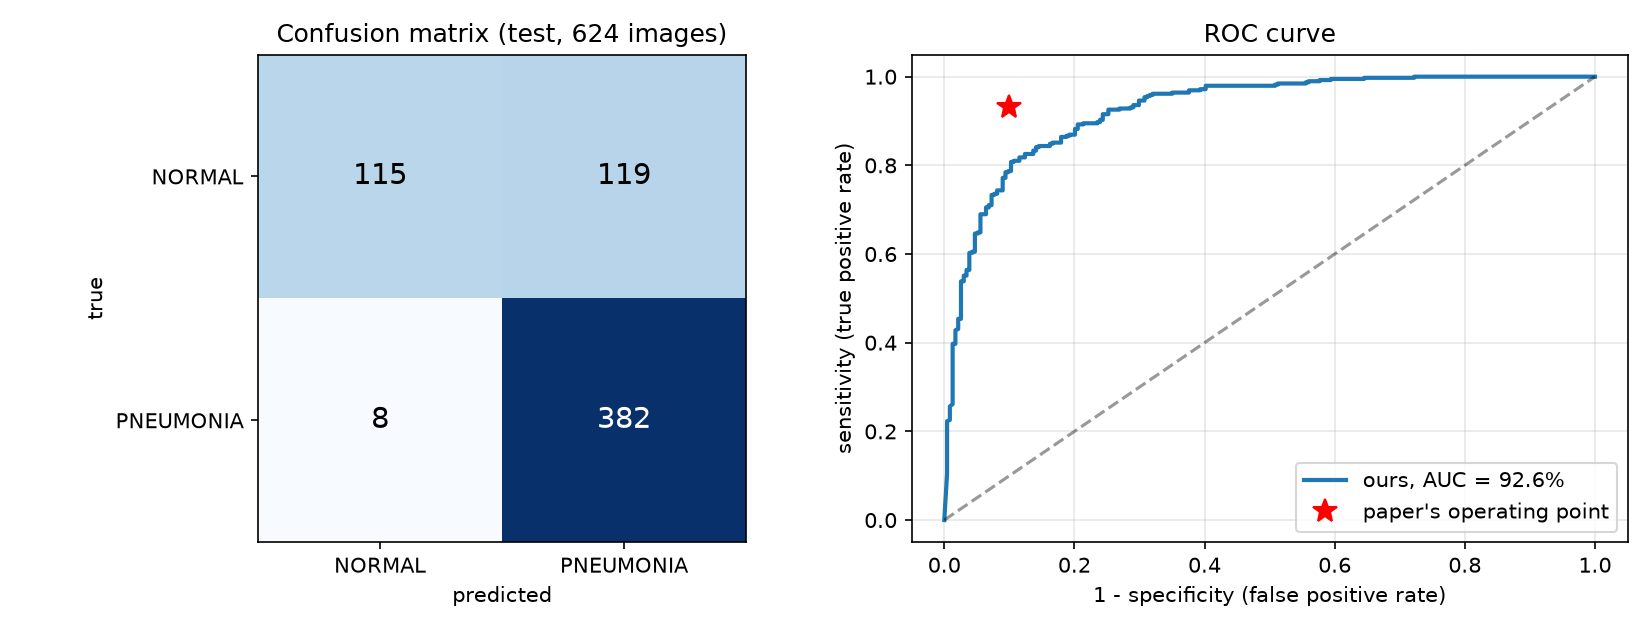
\includegraphics[width=\columnwidth]{confusion_roc.png}
\caption{Frozen baseline, seed 0: confusion matrix on the 624 test images and ROC curve.}
\label{fig:cm}
\end{figure}

\subsection{Ablation: how much of the network to fine-tune}
Table~\ref{tab:ablation} reports the ablation. All rows share the same data, preprocessing and evaluation; the 0-block row is re-run inside the Milestone 4 pipeline (cached in float16), so it can differ slightly from Table~\ref{tab:repro}. ``Train'' is accuracy on the 90\% training portion.

\begin{table*}[t]
\centering
\caption{Ablation over the number of unfrozen Inception blocks (test set, \%, mean$\pm$std where more than one seed).}
\label{tab:ablation}
\begin{tabular}{@{}lcccccccc@{}}
\toprule
Unfrozen & Seeds & Accuracy & Sensitivity & Specificity & Precision & ROC-AUC & Train acc. & Val. acc. \\
\midrule
0 blocks (paper method) & \AblZeroSeeds & \AblZeroAcc & \AblZeroSens & \AblZeroSpec & \AblZeroPrec & \AblZeroAUC & \AblZeroTrain & \AblZeroVal \\
1 block (Mixed\_7c) & \AblOneSeeds & \AblOneAcc & \AblOneSens & \AblOneSpec & \AblOnePrec & \AblOneAUC & \AblOneTrain & \AblOneVal \\
2 blocks (ours) & \AblTwoSeeds & \AblTwoAcc & \AblTwoSens & \AblTwoSpec & \AblTwoPrec & \AblTwoAUC & \AblTwoTrain & \AblTwoVal \\
Whole network$^*$ & \AblAllSeeds & \AblAllAcc & \AblAllSens & \AblAllSpec & \AblAllPrec & \AblAllAUC & \AblAllTrain & \AblAllVal \\
\bottomrule
\end{tabular}\\[2pt]
\footnotesize{$^*$Smaller training budget (batch 32, 1\,000 steps); not directly comparable to the other rows.}
\end{table*}

\IfFileExists{../results/ablation.png}{%
\begin{figure*}[t]
\centering
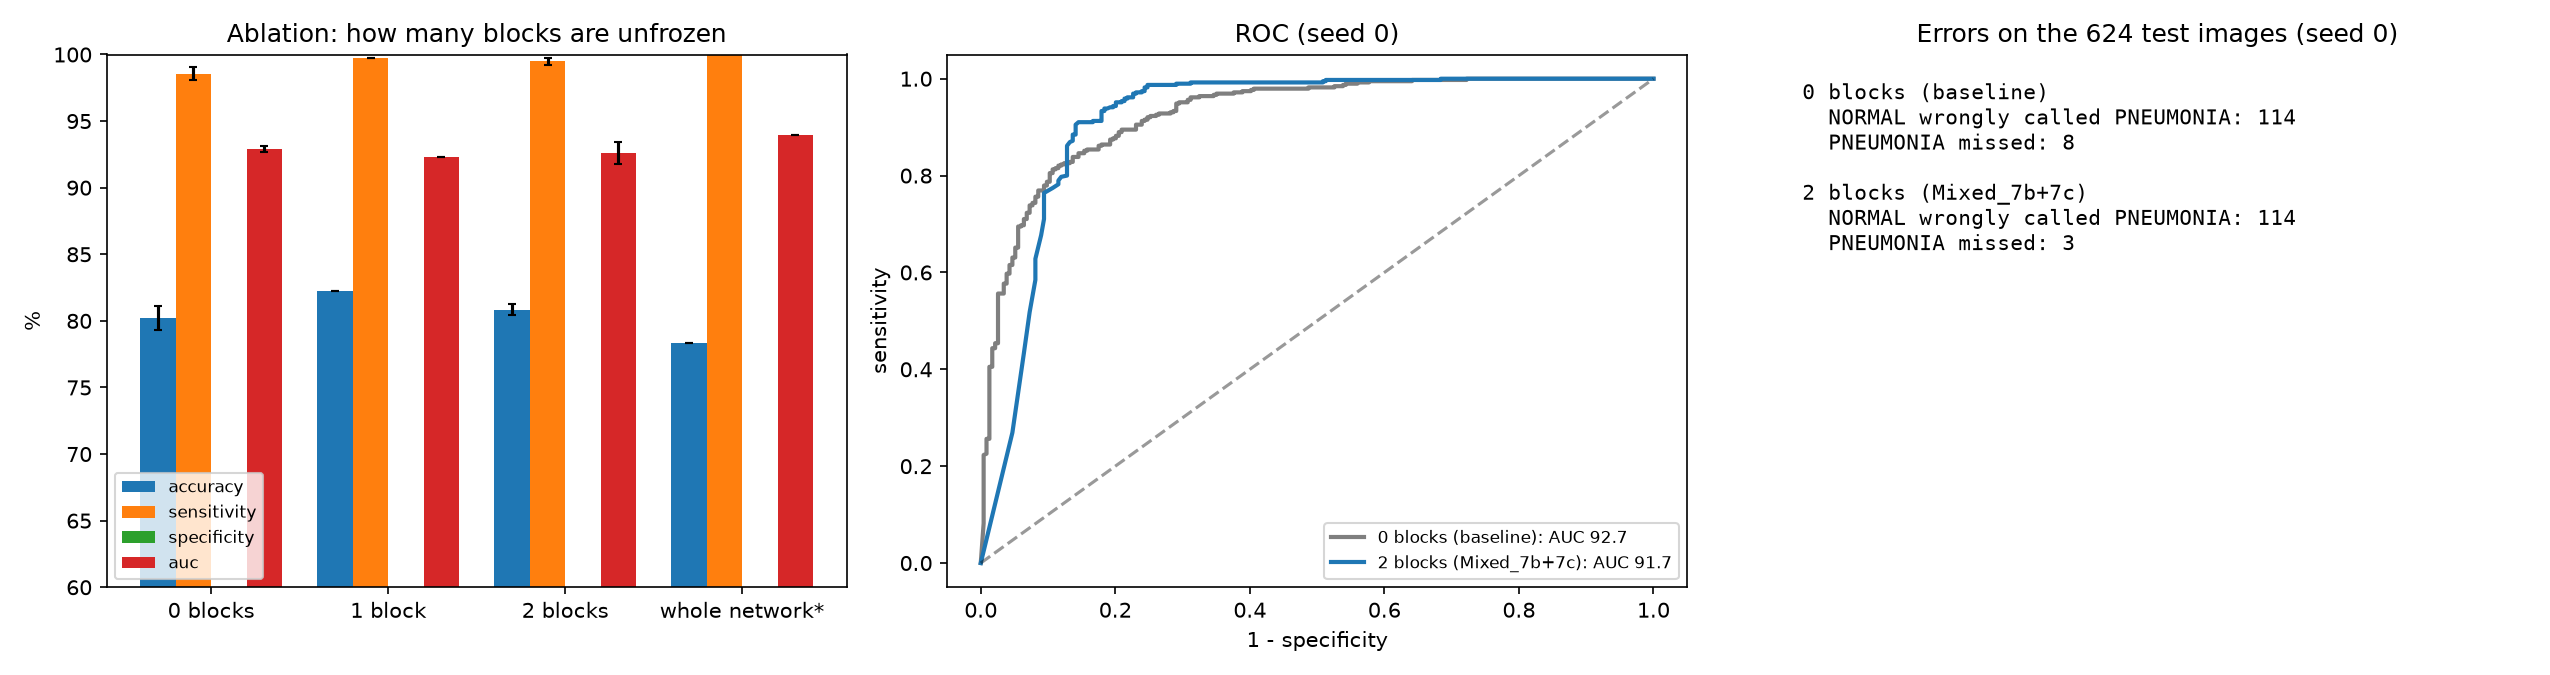
\includegraphics[width=\textwidth]{ablation.png}
\caption{Left: metrics per ablation setting. Middle: ROC of the frozen baseline vs.\ 2 blocks unfrozen (seed 0). Right: test errors of both models (seed 0).}
\label{fig:ablation}
\end{figure*}}{}

% ===========================================================================
\section{Failure Analysis}
\label{sec:fail}
\textbf{Errors are false positives on NORMAL images.} For the frozen baseline (seed 0), 119 of the 127 test errors are NORMAL images predicted as PNEUMONIA; only 8 pneumonia cases are missed (Fig.~\ref{fig:cm}). With 2 blocks fine-tuned, seed 0 makes \FPTwo\ false positives and \FNTwo\ false negatives (baseline in the same pipeline: \FPZero\ and \FNZero). Fig.~\ref{fig:fails} shows the fine-tuned model's most confident mistakes.

\textbf{Train/test distribution shift.} On held-out training images the frozen model reaches 98.66\% validation accuracy, but only 79.65\% on the test set (seed 0). Validation and training images come from the same pool, while the official test set was collected and labelled separately. A model that is near-perfect on one and 19 points worse on the other is learning cues that do not carry over; this is the kind of shift Zech \emph{et al.}~\cite{zech} warn about.

\textbf{Threshold.} At 0.5 the model is strongly biased towards PNEUMONIA. Moving along the same ROC curve to the paper's operating sensitivity (93.6\%, threshold 0.945) gives a specificity of 70.9\% instead of 49.7\%. The paper does not state its threshold or how the final checkpoint was chosen, so part of the gap may be an operating-point choice rather than a weaker model; the remaining AUC gap (92.9 vs.\ 96.8) is not explained by the threshold.

\textbf{Class imbalance.} With about three pneumonia images per normal one and no class weighting, the cross-entropy loss is dominated by pneumonia examples, which pushes predicted probabilities upwards and makes false positives the cheap error during training.

\textbf{Other implementation differences.} We use torchvision's InceptionV3 weights rather than the 2015 TensorFlow graph, PIL bilinear resizing rather than TensorFlow's, and our own random validation split. Any of these can move features and therefore results by a few points.

\IfFileExists{../results/failures_finetuned.png}{%
\begin{figure}[t]
\centering
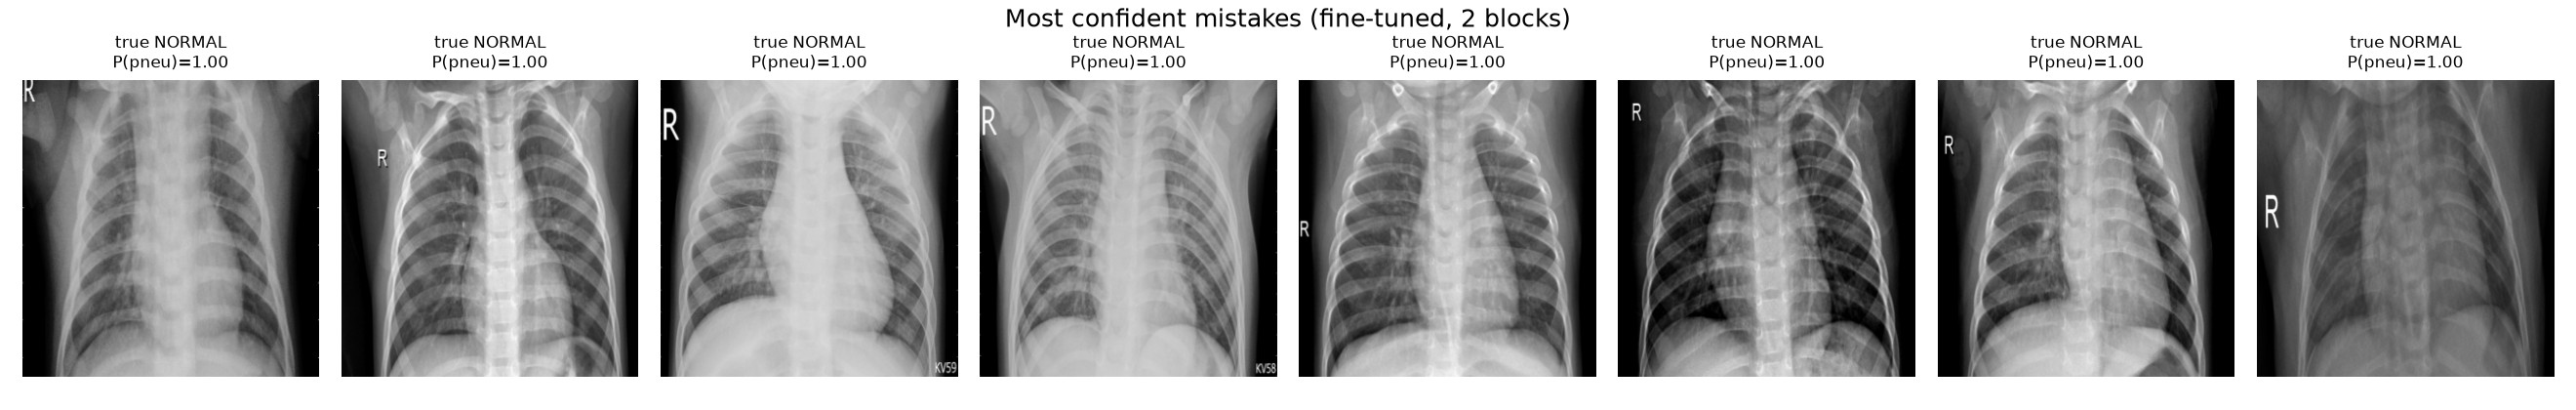
\includegraphics[width=\columnwidth]{failures_finetuned.png}
\caption{Most confident test mistakes of the 2-block fine-tuned model (seed 0), with $P(\text{pneumonia})$.}
\label{fig:fails}
\end{figure}}{%
\begin{figure}[t]
\centering
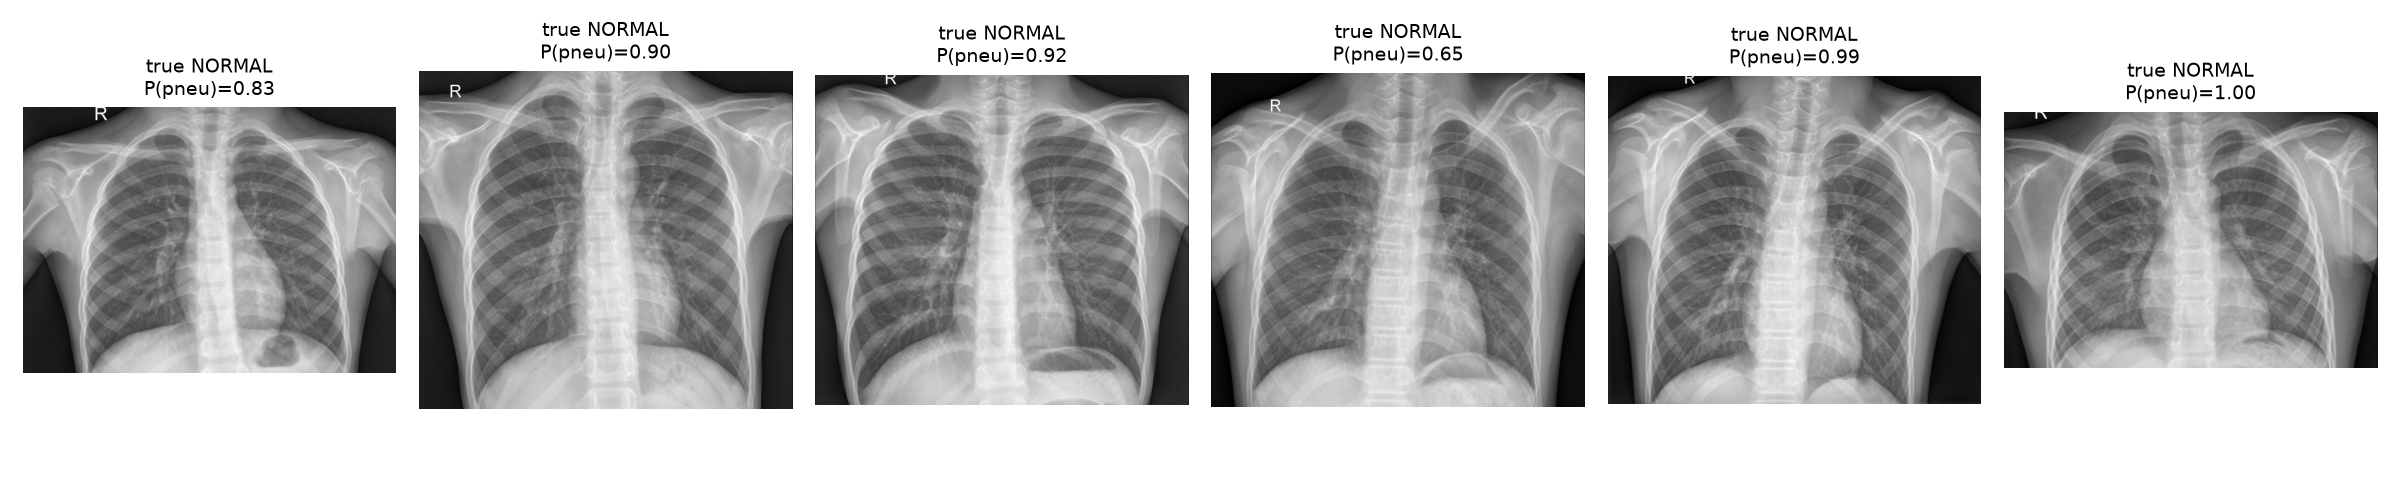
\includegraphics[width=\columnwidth]{failures.png}
\caption{Misclassified test images of the frozen baseline (seed 0). [Fine-tuned failures figure pending.]}
\label{fig:fails}
\end{figure}}

% ===========================================================================
\section{Hypothesis Outcome}
Before running Milestone 4 we predicted (Milestone 3) that unfreezing Mixed\_7b and Mixed\_7c would (a) raise AUC by about 1--2 points, (b) improve specificity more than any other metric, and (c) keep sensitivity within about 1 point. We also stated that the hypothesis is falsified if the AUC gain is $\le$0 or within seed noise, if AUC rises without a specificity gain, or if training accuracy rises while test performance falls.

\begin{table}[t]
\centering
\caption{Pre-registered predictions vs.\ outcome (2 blocks minus frozen, mean over seeds, percentage points).}
\label{tab:outcome}
\begin{tabular}{@{}llc@{}}
\toprule
Prediction & Observed & Verdict \\
\midrule
AUC $+$1--2 & \DAUC & \VerdictAUC \\
Specificity improves most & \DSpec & \VerdictSpec \\
Sensitivity within $\sim$1 & \DSens & \VerdictSens \\
\midrule
Accuracy (not predicted) & \DAcc & -- \\
\bottomrule
\end{tabular}
\end{table}

\OutcomeSummary\ An AUC gain counts as real only if it exceeds both 0.5 points and twice the across-seed standard deviation of the baseline AUC. Table~\ref{tab:ablation} also lets us check the overfitting criterion directly: training accuracy of the fine-tuned models (\AblTwoTrain\% for 2 blocks) should be compared with their test accuracy (\AblTwoAcc\%). Because only \AblTwoSeeds\ seeds were run for 2 blocks, this conclusion is weaker than the reproduction result.

% ===========================================================================
\section{Limitations}
\begin{itemize}
\item One dataset from one hospital and a single fixed test set of 624 images; no external validation.
\item Few seeds for the fine-tuned configurations (1--2), and the whole-network row uses a smaller training budget.
\item We could not fully verify the paper's reported sensitivity, specificity and AUC, nor its threshold and checkpoint selection.
\item A fixed 0.5 threshold is used for all models; no calibration or class weighting.
\item No data augmentation was used, to stay faithful to the baseline.
\item This is a course reproduction study. The models are not validated for, and must not be used in, any clinical setting.
\end{itemize}

% ===========================================================================
\section{Conclusion}
We reproduced the frozen-InceptionV3 pneumonia classifier of Kermany \emph{et al.} and obtained a high sensitivity but a much lower specificity and a 3.9-point lower AUC than reported. The shortfall is concentrated in false positives on NORMAL images and is linked to a train/test distribution shift, class imbalance and the default threshold. Fine-tuning the top two Inception blocks changed AUC by \DAUC\ points and specificity by \DSpec\ points, and our pre-registered hypothesis is \VerdictOverall. Natural next steps are class-weighted loss, choosing the threshold on validation data, X-ray-appropriate augmentation, more seeds, and testing on an external dataset.

% ===========================================================================
\begin{thebibliography}{99}
\bibitem{who} World Health Organization, ``Pneumonia in children,'' Fact sheet, Nov.~11, 2022. [Online]. Available: \url{https://www.who.int/news-room/fact-sheets/detail/pneumonia}

\bibitem{kermany} D.~S. Kermany \emph{et al.}, ``Identifying medical diagnoses and treatable diseases by image-based deep learning,'' \emph{Cell}, vol.~172, no.~5, pp.~1122--1131, 2018, doi: 10.1016/j.cell.2018.02.010.

\bibitem{chexnet} P.~Rajpurkar \emph{et al.}, ``CheXNet: Radiologist-level pneumonia detection on chest X-rays with deep learning,'' arXiv:1711.05225, 2017.

\bibitem{yosinski} J.~Yosinski, J.~Clune, Y.~Bengio, and H.~Lipson, ``How transferable are features in deep neural networks?,'' in \emph{Advances in Neural Information Processing Systems 27 (NIPS)}, 2014, pp.~3320--3328.

\bibitem{raghu} M.~Raghu, C.~Zhang, J.~Kleinberg, and S.~Bengio, ``Transfusion: Understanding transfer learning for medical imaging,'' in \emph{Advances in Neural Information Processing Systems 32 (NeurIPS)}, 2019.

\bibitem{mendeley} D.~Kermany, K.~Zhang, and M.~Goldbaum, ``Labeled optical coherence tomography (OCT) and chest X-ray images for classification,'' Mendeley Data, v2, 2018, doi: 10.17632/rscbjbr9sj.2.

\bibitem{inception} C.~Szegedy, V.~Vanhoucke, S.~Ioffe, J.~Shlens, and Z.~Wojna, ``Rethinking the Inception architecture for computer vision,'' in \emph{Proc. IEEE Conf. Computer Vision and Pattern Recognition (CVPR)}, 2016, pp.~2818--2826.

\bibitem{imagenet} J.~Deng, W.~Dong, R.~Socher, L.-J. Li, K.~Li, and L.~Fei-Fei, ``ImageNet: A large-scale hierarchical image database,'' in \emph{Proc. IEEE Conf. Computer Vision and Pattern Recognition (CVPR)}, 2009, pp.~248--255.

\bibitem{chestxray8} X.~Wang, Y.~Peng, L.~Lu, Z.~Lu, M.~Bagheri, and R.~M. Summers, ``ChestX-ray8: Hospital-scale chest X-ray database and benchmarks on weakly-supervised classification and localization of common thorax diseases,'' in \emph{Proc. IEEE Conf. Computer Vision and Pattern Recognition (CVPR)}, 2017, pp.~2097--2106.

\bibitem{zech} J.~R. Zech, M.~A. Badgeley, M.~Liu, A.~B. Costa, J.~J. Titano, and E.~K. Oermann, ``Variable generalization performance of a deep learning model to detect pneumonia in chest radiographs: A cross-sectional study,'' \emph{PLoS Medicine}, vol.~15, no.~11, e1002683, 2018.

\bibitem{adam} D.~P. Kingma and J.~Ba, ``Adam: A method for stochastic optimization,'' in \emph{Proc. Int. Conf. Learning Representations (ICLR)}, 2015.

\bibitem{pytorch} A.~Paszke \emph{et al.}, ``PyTorch: An imperative style, high-performance deep learning library,'' in \emph{Advances in Neural Information Processing Systems 32 (NeurIPS)}, 2019, pp.~8024--8035.
\end{thebibliography}

\end{document}
